\documentclass[]{article}

\usepackage{graphicx}

%opening
\title{How do adaptive radiations sustain themselves?}
\author{Rapha\"{e}l Scherrer, G. Sander van Doorn, Rampal S. Etienne}

\begin{document}

\maketitle

\begin{abstract}

Adaptive radiations are bursts of new species occuring over a short period of geological time. Major examples include Anolis lizards from the Caribbean or East African cichlid fish. Although adaptive radiations have attracted much attention and research effort, in search for insight into the process of species diversification, they remain a rather anomalous case throughout the tree of life, that is yet to be fully explained by theory. In particular, current speciation theory predicts that if competitive interactions are a major force driving species to diverge, and if gene flow tends to slow down the rise of reproductive isolation until strong postzygotic barriers arise, then speciation events should be more rare than observed in adaptive radiations, and successive events should be separated by increasing periods of time towards the present. That is, previous speciation events should delay further speciation events, primarily because of a weakening of selective pressures. In contrast, adaptive radiations are marked by a sustained high rate of speciation, resulting in branching closely clustered branching points over a short period of time. Here, we propose a model that implements some of the mechanisms that have been invoked to explain this pattern. These include (1) the maintenance of protected genetic diversity prior to the radiation (through e.g. past demographic history or balancing selection), which can be recruited to fuel rapid adaptation, (2) the presence of external, environmentally imposed discrete ecological niches and little reliance on frequency-dependent competition, and (3) genetic assimilation from a highly plastic ancestor. To accomodate these various scenarios, we developed an individual-based simulation of a sexually reproducing, diploid species with an explicit, mutating genome consisting of numerous loci coding for multiple traits, which in turn determine fitness in an adaptive landscape composed of multiple peaks, or niches. Recombination allows gene flow and introgression between the incipient species. Reproductive isolation can occur through prezygotic, behavioral barriers, by means of evolving mating cues and non-costly mate preference and sexual selection. This assumes, as proposed by previous authors, that the dimensionality of mating cues is non-limiting for subsequent speciation events, that is, there are enough ways sexual cues can diversify for every pair of species to be able to tell each other apart (guess a whole paper could be written about just that? Last chapter of Sander's thesis?). We found that...

\end{abstract}

\section*{Introduction}

\subsection*{Questions}

\begin{enumerate}

	\item How does the influence of ecology (e.g. niche width relative to competition kernel) on whether diversification occurs change with a higher dimensionality of phenotype space and spatial heterogeneity? This is related to the idea of a percolation threshold, where a tipping point may exist in ecological conditions such a generalist species is favored on one side of it, while on the other side an explosive radiation arises. Such a model could test this hypothesis in relation to phenotypic dimensionality and spatial heterogeneity, for example.
	
	\item Using its explicit genetics, can we test the hypothesis that rapid radiations arise thanks to the presence of a large genetic diversity in the ancestral population, which, upon some event (to be defined) becomes involved in rapid adaptive diversification? A large genetic diversity prior to radiation has been invoked to explain the explosive diversification of cichlids, for example. Mechanisms leading to such large genetic variation include (a) the accumulation of neutral diversity in multiple demographic cycles of fission (accumulation of new mutations in allopatry) and fusion (hybridization and recombination) of populations, (b) widespread protected polymorphisms across the genome, mediated by balancing selection, or (c) phenotypic plasticity in the ancestral population, where genetic variation is protected from selection. How this genetic variation that is protected from selection becomes involved in genetic differentiation is not clear though. Genetic assimilation from a plastic ancestor is one potential mechanism.	 
	
\end{enumerate}

\section*{Model}

\begin{figure}
	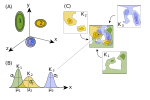
\includegraphics[width=\textwidth]{./figures/model_overview/model.png}
	\caption{Model overview}
	\label{fig:overview}
\end{figure}

The model is an individual-based simulation. We consider an initial population of a diploid, sexually reproducing species. The life cycle consists in a phase of competition for the resources, followed by reproduction, then survival (generations can be overlapping), and finally dispersal across the geographically explicit landscape.\\

The landscape takes the form of a biogeographical region; a large grid with spatial heterogeneity of resources or habitats. This spatial heterogeneity implies that local conditions differ across the landscape and different phenotypes may be advantageous in different places.\\

In every location, some resources may be present. A resource can be viewed as a niche in the phenotypic space of the species (whose dimensionality must be set at the beginning of the simulation). This niche in turn symbolizes the combination of trait values that are needed to optimally assimilate that resource. How many different resources there are, where they are located in phenotype space, and how wide their respective niche is, may be provided by the user. Specifically, the user provides the number of dimensions $D$ of phenotype space, and the number of ecological niches $N$. Niches are modeled as multivariate Gaussian functions (Figure \ref{fig:overview}), with locations in phenotype space (i.e. multivariate means) and niche breadth (i.e. variance) sampled from a certain distribution, with parameters provided by the user. The abundance of each resource, $K$, varies through geographical space (Fig. \ref{fig:overview}) according to a perlin noise generator (or any algorithm that generates spatial heterogeneity?).\\

Resources are present in limited amounts, and in order to acquire them, individuals must compete, even more so that they are close in phenotype space. Negative frequency-dependence is generated this way. A competition kernel parameter for each dimension can tune this. The amount of resources secured by individuals translates into a fitness value, or reproductive success.\\

Reproduction is sexual. The idea is that species become reproductively isolated from each other as they diverge. One way of promoting this process is to allow for postzygotic incompatibilities. These can arise from a low fitness of hybrid phenotypes given certain environmental conditions (i.e. intermediate hybrids not well adapted to either of their parental niches), but also from internal, developmental or genomic incompatibilities, which can be implemented in the genome in the form of Dobzhansky-Muller incompatibilities. That said, such incompatibilities may not necessarily be neutral (as in DM) but may also involve loci coding for some ecological traits.\\

Reduced fitness of hybrids is generally thought to promote the evolution of prezygotic barriers. These can take many forms, from behavioral preferences to mismatches in copulatory organs or molecular recognition systems. There are multiple ways to model this. One way is to give individuals, in addition to ecological traits determining the niches they can adapt to, some sexual cues expressed in one sex (e.g. males), and some preferences expressed in the other, choosy sex (e.g. females). These three categories of traits may be independent of each other, but in this case, (adaptive) speciation is unlikely to occur because recombination will typically break the linkage between ecological and sexual loci, making reproductive isolation not match the ecotype boundaries. This problem can be solved by linking either the mating cue or the mating preference to the trait involved in ecological divergence, thus making the ecological trait a magic trait, or a magic preference, respectively. Finally, all three types of traits can be combined into one trait involved in ecology, sexual display and sexual preference, into a so-called phenotype-matching model. These conditions should allow reproductive isolation to happen. A simpler version of the model could have a fixed assortative mating parameter, instead of an evolving mate choice.\\

A fitness landscape with multiple resources / niches, together with a heterogeneous spatial structure, frequency-dependent selection and ecologically-mediated sexual selection, should promote the establishment of post- and prezygotic barriers to gene flow, and thus speciation. However, to get repeated speciation events some other aspects must be considered. One is the dimensionality of the sexual phenotype space. Indeed, if divergence in sexual trait or sexual preference must arise for prezygotic isolation to happen, it is likely that the number of dimensions along which such trait can diversify will influence the number of reproductively isolated species that can occur. It has been argued in the literature that in explosive radiations the dimensionality of sexual space is not limiting.\\

Another important aspect of our model is that it must allow us to test proposed theories for the occurrence of rapid radiations. One theory is that important amounts of accumulated cryptic genetic variation are present at the onset of radiations, and become recruited in ecological adaptation. A large genetic diversity prior to radiation has been invoked to explain the explosive diversification of cichlids, for example. Mechanisms leading to such large genetic variation include (a) the accumulation of neutral diversity in multiple demographic cycles of fission (accumulation of new mutations in allopatry) and fusion (hybridization and recombination) of populations, (b) widespread protected polymorphisms across the genome, mediated by balancing selection, or (c) phenotypic plasticity in the ancestral population, where genetic variation is protected from selection. How this genetic variation that is protected from selection becomes involved in genetic differentiation is not clear though. Genetic assimilation from a plastic ancestor is one potential mechanism. Fluctuations in niche space through time (i.e. what combinations of trait values yield a high fitness) may have to be involved.\\

More complex genetic scenarios such as pleiotropy, non-additive genetics or structural mutations (e.g. inversions, duplications) may be relevant but too complicated.

\section*{Results}

\section*{Discussion}

\end{document}
